\documentclass[crop,tikz]{standalone}
\usetikzlibrary{backgrounds}
\colorlet{blue}{cyan}
\tikzset{ inverted/.style={every path/.style={draw=white,text=white}, background rectangle/.style={fill}, show background rectangle }}

\tikzset{>=latex}

\begin{document}
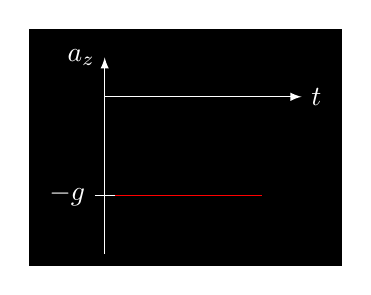
\begin{tikzpicture}[inverted,scale=2.5]
  \draw[->] (0,0) -- (1,0) node[right] {$t$};
  \draw[->] (0,-0.8) -- (0,0.2) node[left] {$a_z$};
  \draw[red] (0,-0.5) -- (0.8,-0.5);
  \draw (-0.05,-0.5) node[left] {$-g$} -- (0.05,-0.5);
\end{tikzpicture}
\end{document}
